\documentclass[12pt,spanish]{article}
\usepackage[spanish]{babel}
\usepackage{graphicx}
\usepackage{color}
\usepackage{xcolor}
\usepackage{colortbl}
\usepackage{amsthm,thmtools}
\usepackage{dirtytalk}
\usepackage{multirow}
\usepackage{amsmath}
\usepackage{subcaption}
\usepackage{adjustbox}
\usepackage{amsmath}
\usepackage{centernot}
\usepackage{mathtools}
\usepackage{multirow}
\usepackage[hidelinks]{hyperref}
\usepackage{caption}
\usepackage{eurosym} % para el euro
\usepackage{amsthm}
\usepackage{multicol}
\usepackage{float}
\usepackage{amsfonts}
\usepackage{titling}
\usepackage{soul}
\usepackage{listings}
\usepackage{array}
\usepackage{tikz}
\usetikzlibrary{shapes.geometric, arrows, chains, calc,positioning,fit,decorations.pathreplacing}
\usepackage[framemethod=tikz]{mdframed}

\graphicspath{ {../../img/}}
\selectlanguage{spanish}
\usepackage[utf8]{inputenc}
\usepackage{graphicx}
\usepackage[a4paper,left=3cm,right=2cm,top=2.5cm,bottom=2.5cm]{geometry}

\newenvironment{solution}{
	\par
	\textbf{Solución}
	\par
	\begin{center}
}
{
	\end{center}
}

\lstset{
  breaklines=true,
  postbreak=\mbox{\textcolor{red}{$\hookrightarrow$}\space},
}


\title{Servidores Web de Altas Prestaciones}
\setlength{\droptitle}{10em}
\author{Carlos Sánchez Páez}

\makeindex
\begin{document}
\definecolor{light-gray}{gray}{0.95}
\lstset{columns=fullflexible,basicstyle=\ttfamily}
\surroundwithmdframed[
  hidealllines=true,
  backgroundcolor=light-gray,
  innerleftmargin=0pt,
  innertopmargin=0pt,
  innerbottommargin=0pt]{lstlisting}


\begin{titlepage}

 \newlength{\centeroffset}
 \setlength{\centeroffset}{-0.5\oddsidemargin}
 \addtolength{\centeroffset}{0.5\evensidemargin}
 \thispagestyle{empty}

 \noindent\hspace*{\centeroffset}
 \begin{minipage}{\textwidth}

  \centering
  
\includegraphics[width=0.9\textwidth]{logo_ugr.jpg}\\[1.4cm]

  \textsc{ \Large Servidores Web de Altas Prestaciones\\[0.2cm]}
  \textsc{GRADO EN INGENIERÍA INFORMÁTICA}\\[1cm]

  {\Huge\bfseries Instalación de GOBetween \\}
 \end{minipage}

 \vspace{1.5cm}
 \noindent\hspace*{\centeroffset}
 \begin{minipage}{\textwidth}
  \centering

  \textbf{Autor}\\ {Carlos Sánchez Páez}\\[2.5ex]
  
\includegraphics[width=0.4\textwidth]{etsiit_logo.png}\\[0.1cm]
  \vspace{1.5cm}
  
\includegraphics[width=0.15\textwidth]{atc.jpg}\\[0.1cm]
  \vspace{1cm}
  \textsc{Escuela Técnica Superior de Ingenierías Informática y de Telecomunicación}\\
  \vspace{1cm}
  \textsc{Curso 2019-2020}
 \end{minipage}
\end{titlepage}
\thispagestyle{empty}
\newpage
\tableofcontents{}
\newpage


En esta tarea instalaremos GOBetween en M3 y la configuraremos como balanceador de carga.

\begin{enumerate}
	\item Paramos el balanceador de carga que tengamos activo:
	\begin{lstlisting}
	m3 > sudo systemctl stop <haproxy|nginx>
	\end{lstlisting}
	\item Instalamos GOBetween:
	\begin{lstlisting}
	m3 > sudo snap install gobetween --edge
	\end{lstlisting}
	\item Modificamos el archivo de configuración:
	\begin{lstlisting}
	m3 > sudo nano /var/snap/gobetween/common/gobetween.toml
	\end{lstlisting}
	Añadimos las siguientes líneas:
	\begin{lstlisting}
	[servers.servidoresSWAP]
		bind = "192.168.56.104:80"
		protocol = "tcp"
		balance = "roundrobin"

		max_connections = 10000
		client_idle_timeout = "10m"
		backend_idle_timeout = "10m"
		backend_connection_timeout = "2s"

	[servers.servidoresSWAP.discovery]
		kind = "static"
		static_list = [
		        "192.168.56.100:80",
		        "192.168.56.103:80"
		]
	\end{lstlisting}
	\item Ejecutamos el balanceador y comprobamos su funcionamiento:
	\begin{lstlisting}
	m3 > sudo snap run gobetween
	\end{lstlisting}
	\begin{figure}[H]
		\centering
		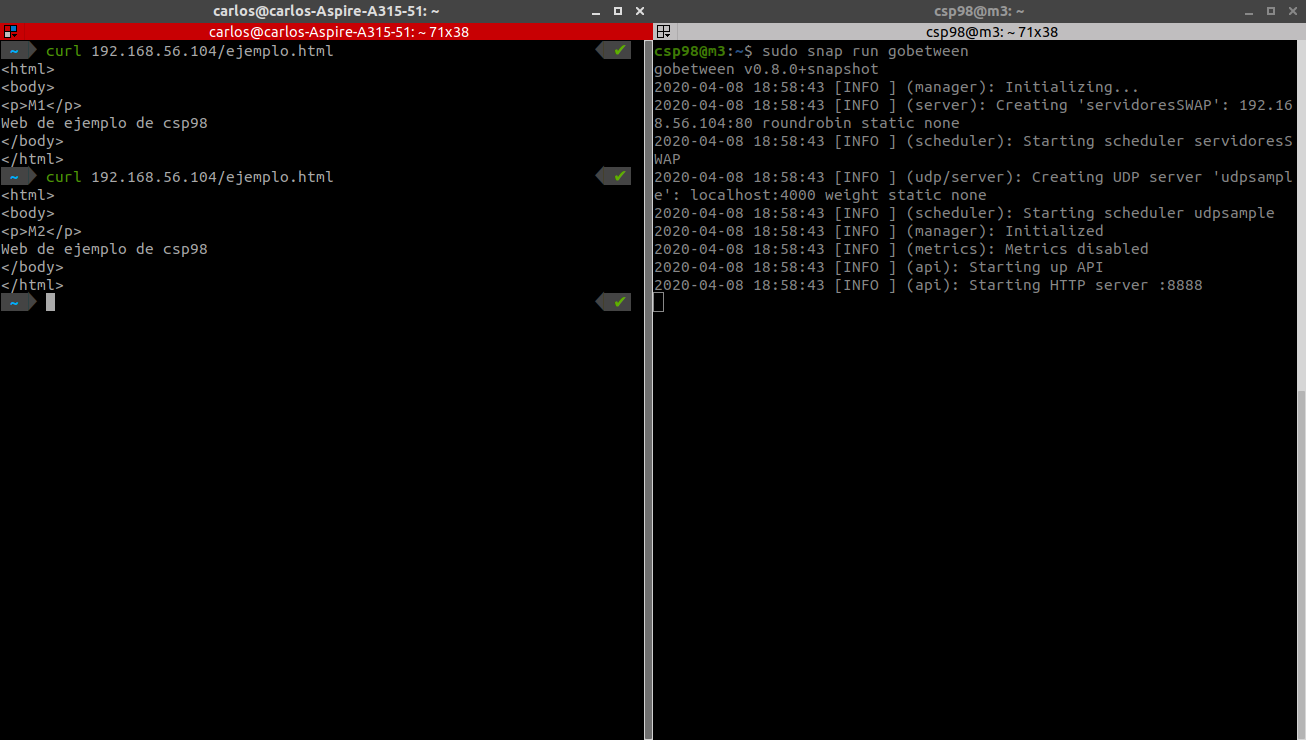
\includegraphics[scale=0.45]{t4/gobetween-ok.png}
	\end{figure}
\end{enumerate}

Este balanceador de carga es sencillo de configurar, al igual que \emph{nginx} y \emph{haproxy}.


\end{document}
